
\begin{frame}
\frametitle{Image Locatization}
Second step:
\begin{itemize}
\item find bounding boxes of images on new books
\item classify whether patch is an image or text patch
\item reconstruct images from patches
\end{itemize}
HOG features:
\begin{itemize}
\item 10x20 per page
\item Additionally: concatenate features, 9x19 per page
\end{itemize}
\end{frame}

\subsection{Method}
\begin{frame}
\frametitle{Conditional Random Fields (CRF)}
\begin{itemize}
\item Regard image patches, and their labels, as an undirected graph (labels $x_i$, patches $y_i$)
\item Decide label $x_i$ on patch likeliness, neighborhood, and prior
\item Solver: Structural Support Vector Machine (SSVM)
\end{itemize}
$$ E(\mathbf{x}, \mathbf{y}) = h\sum_i x_i - \beta \sum_{\{i, j\}} x_i x_j
- \eta \sum_i x_i y_i $$

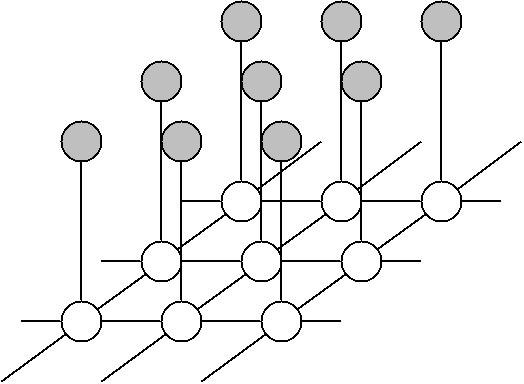
\includegraphics[width=.3\paperwidth]{resources/crf}
\end{frame}

\begin{frame}{CRF and SSVM}

\begin{itemize}
\item To solve the CRF, the energy function must be minimized.
\item For this, two types of SSVMs can be used:
\begin{itemize}
	\item N-slack SSVM
	\item One-slack SSVM
\end{itemize}
\item $\argmin \hat{y} \text{E}(x, y) + \text{loss}(\hat{y}, y) $
\item Where the loss is the \emph{Hamming} loss
\end{itemize}
\end{frame}

\begin{frame}
\frametitle{Preprocess Features Using an SVM}
\begin{itemize}
\item HOG features have 8 values
\item SSVM is harder to solve for more dimensions per feature
\item Use SVM to assign confidence score to each feature
\item Now SSVM has input of 1 dimension per feature
\end{itemize}
\end{frame}

\begin{frame}
\frametitle{Two Stage Training}
Require two stage training to prevent overfitting.
\begin{itemize}
\item Train SVM on $75\%$ of train set, and predict labels on remainder for SSVM
\item Repeat 4 times, with different splits
\item Now $100\%$ of the SSVM features is available
\item Once more: train SVM on $100\%$ of train set to obtain best model
\end{itemize}
\begin{center}
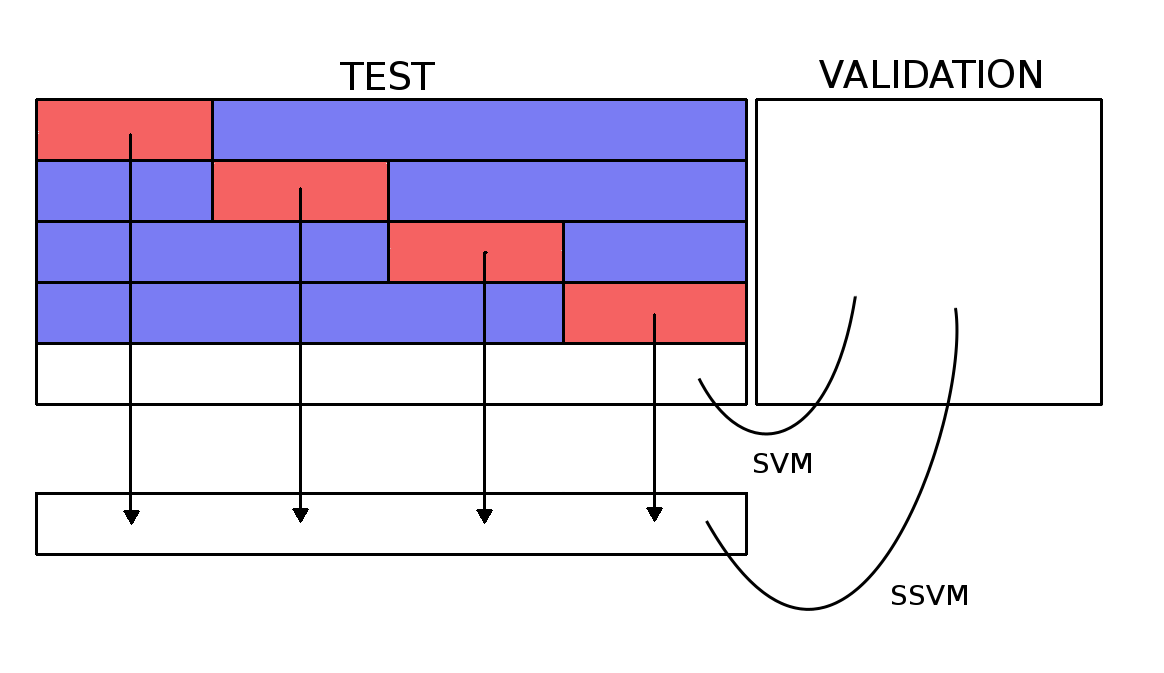
\includegraphics[width=.5\paperwidth]{resources/twostage}
\end{center}
\end{frame}

\subsection{Results}


\begin{frame}
\frametitle{Results, Single Features}

\begin{block}{Scores}
\begin{tabular}{l l l  | l l}
 & \multicolumn{2}{c}{\emph{Pre-trained}} & \multicolumn{2}{c}{\emph{Direct}} \\
& \textbf{Image} & \textbf{Text} & \textbf{Image} & \textbf{Text} \\
\textbf{Precision} & 0.271 & 0.979 & 0.271 & 0.979 \\
\textbf{Recall} & 0.700 & 0.884 & 0.700 & 0.884 \\
\textbf{F-score} & 0.391 & 0.929 & 0.391 & 0.929
\end{tabular}
\end{block}

\begin{block}{Confusion matrices}
\begin{tabular}{l l l | l l }
& \multicolumn{2}{c}{\emph{Pre-trained}} & \multicolumn{2}{c}{\emph{Direct}} \\
Real\textbackslash Predicted & \textbf{Image} & \textbf{Text} & \textbf{Image} & \textbf{Text} \\
\textbf{Image} &  523370&  59995& 523370 & 59995 \\
\textbf{Text} &  562795&  5477440& 562795 & 5477440
\end{tabular}
\end{block}
\end{frame}



\begin{frame}
\frametitle{Results, Concatenated Features}

\begin{block}{Scores}
\begin{tabular}{l l l  | l l}
 & \multicolumn{2}{c}{\emph{Pre-trained}} & \multicolumn{2}{c}{\emph{Direct}} \\
  & \textbf{Image} & \textbf{Text} & \textbf{Image} & \textbf{Text} \\
\textbf{Precision} & 0.269 & 0.979 & 0.241 & 0.979 \\
\textbf{Recall} & 0.743 & 0.854 &  0.750 & 0.830 \\
\textbf{F-score} & 0.395 & 0.912 & 0.365 & 0.898
\end{tabular}
\end{block}

\begin{block}{Confusion matrices}
\begin{tabular}{l l l | l l }
& \multicolumn{2}{c}{\emph{Pre-trained}} & \multicolumn{2}{c}{\emph{Direct}} \\
Real\textbackslash Predicted & \textbf{Image} & \textbf{Text} & \textbf{Image} & \textbf{Text} \\
\textbf{Image} & 524523 & 58481 & 524759 & 58245 \\
\textbf{Text} & 566567 & 5390857 & 577927 & 5379497
\end{tabular}
\end{block}



\end{frame}
